\documentclass{article}
\usepackage{graphicx} % Required for inserting images
\input{setup}
\usepackage[margin=2cm]{geometry}
\usepackage{polski}
\title{Nadprzewodnictwo Topologiczne. Fermiony Majorany.}
\author{Marta Wleklińska}
\date{\today}
\newcommand{\opr}[1]{\mathbf{\hat{#1}}}
\begin{document}

\maketitle
%%%%%%%%%%%%%%%%%%%%%%%%%%%%%%%%%%%%%%%%%%%%%%%%%%%
\section{Wstęp}
%%%%%%%%%%%%%%%%%%%%%%%%%%%%%%%%%%%%%%%%%%%%%%%%%%%
W ćwiczeniu analizowaliśmy model Kitaeva oraz układ eksperymentalny w celu zaobserwowania stanów Majorany.
%%%%%%%%%%%%%%%%%%%%%%%%%%%%%%%%%%%%%%%%%%%%%%%%%%%
\section{Wyniki}
%%%%%%%%%%%%%%%%%%%%%%%%%%%%%%%%%%%%%%%%%%%%%%%%%%%
\subsection{Kitaev}
%%%%%%%%%%%%%%%%%%%%%%%%%%%%%%%%%%%%%%%%%%%%%%%%%%%
W pierwszym ćwiczeniu hamiltonian był w postaci
\begin{equation}
    \opr{H} = -\mu \sigma_z \ket{\psi_i}\bra{\psi_i} - t\sigma_z\ket{\psi_i}\bra{\psi_{i+1}}
    -
    t\sigma_z\ket{\psi_i}\bra{\psi_{i-1}}
    +\ii \Delta \sigma_y\ket{\psi_i}\bra{\psi_{i+1}}
    -\ii \Delta \sigma_y\ket{\psi_i}\bra{\psi_{i-1}},
\end{equation}
gdzie $\ket{\psi_i}=(\ket{\psi_i^e \ \ket{\psi_i^h}})$ to wektor na węźle $i$, który składa się z części elektronowej oraz dziurowej, $\mu$~to potencjał chemiczny, $t$ to energia przeskoku między węzłami, a $\Delta$ określa energię parowania elektronowego. 
Po dyskretyzacji mogliśmy zapisać wyrażenie \texttt{onsite} oraz~\texttt{hopping} i zdefiniować układ.
Na rysunku~\ref{fig:kitaev-spectra} przedstawione zostały obliczenia energii stanów w funkcji potencjału chemicznego~$\mu\in[0,4t]$.
\begin{figure}[htp!]
    \centering
    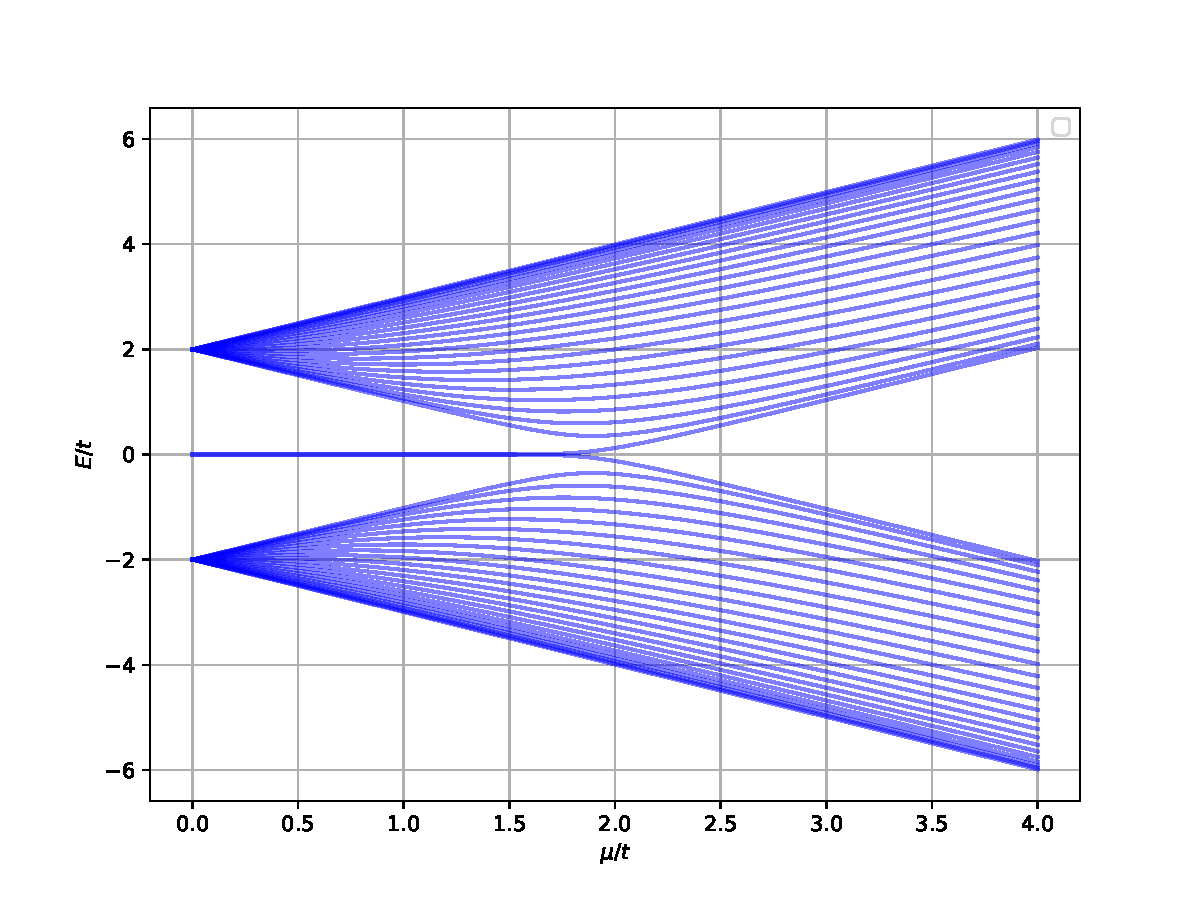
\includegraphics[width=0.65\linewidth]{ex1_spectrum.pdf}
    \caption{Spektrum energii w funkcji $\mu/t.$ Wyniki dla łańcucha Kitaeva}
    \label{fig:kitaev-spectra}
\end{figure}
%%%%%%%%%%%%%%%%%%%%%%%%%%%%%%%%%%%%%%%%%%%%%%%%%%%
Zauważamy stany o zerowej energii dla $\mu<2t$, które odpowiadają stanom Majorany.\\
\\
W kolejnym kroku zapisaliśmy wykres dla stanu o energii najbliższej lub równej zeru dla przypadku $\mu=t$~(rys.~\ref{fig:ex1-density}) i $\mu=4t$~(rys.~\ref{fig:ex1-density4t}).
%%%%%%%%%%%%%%%%%%%%%%%%%%%%%%%%%%%%%%%%%%%%%%%%%%%
\begin{figure}[htp!]
    \centering
    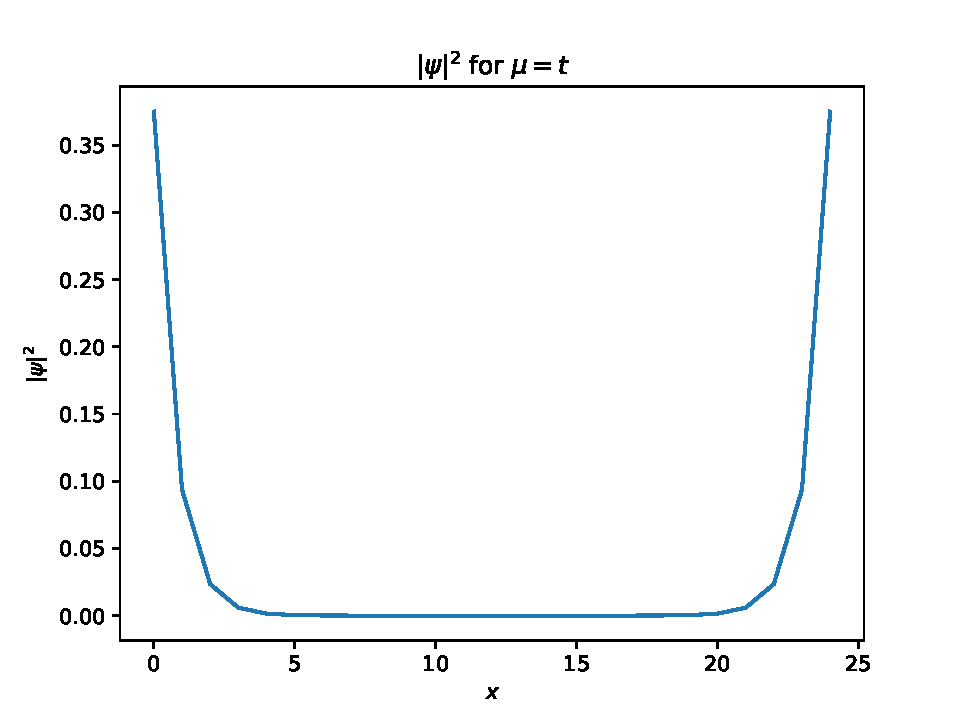
\includegraphics[width=0.65\linewidth]{ex1_density.pdf}
    \caption{Moduł funkcji falowej stanu najbliższego energii $E=0$ dla $\mu=t$. Wyniki dla łańcucha Kitaeva}
    \label{fig:ex1-density}
\end{figure}
%%%%%%%%%%%%%%%%%%%%%%%%%%%%%%%%%%%%%%%%%%%%%%%%%%%
%%%%%%%%%%%%%%%%%%%%%%%%%%%%%%%%%%%%%%%%%%%%%%%%%%%
\begin{figure}[htp!]
    \centering
    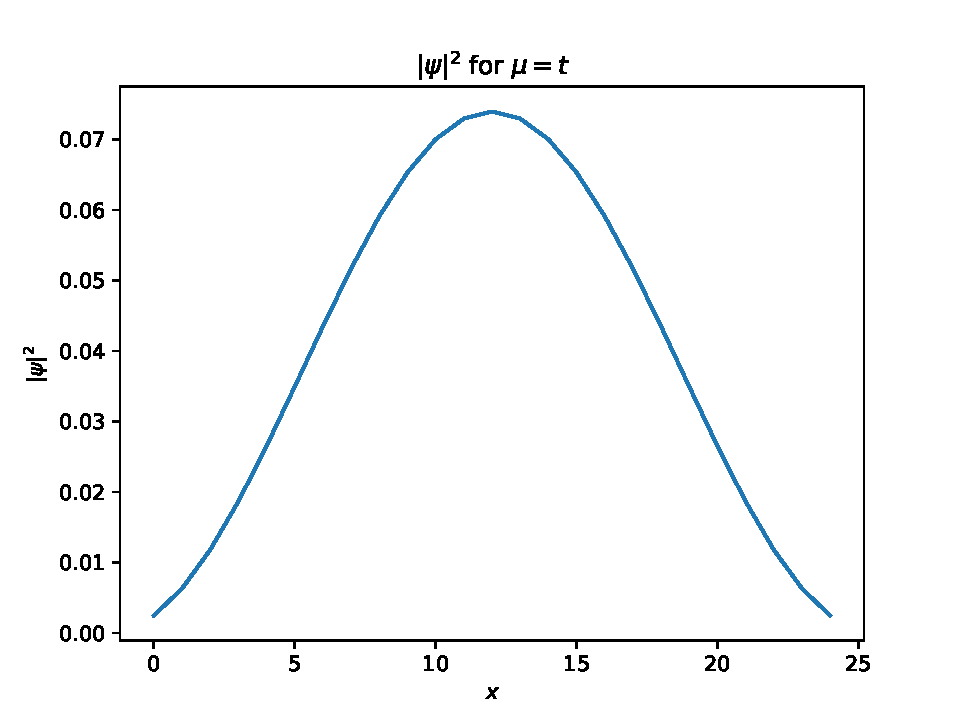
\includegraphics[width=0.65\linewidth]{ex1_density4t.pdf}
    \caption{Moduł funkcji falowej stanu najbliższego energii $E =0$ dla $\mu=4t$. Wyniki dla łańcucha Kitaeva}
    \label{fig:ex1-density4t}
\end{figure}
%%%%%%%%%%%%%%%%%%%%%%%%%%%%%%%%%%%%%%%%%%%%%%%%%%%
Dla $\mu = t$ obserwujemy lokalizację funkcji falowej na końcach łańcucha, co świadczy o obecności stanów Majorany w fazie topologicznej. 
Z kolei dla $\mu = 4t$ rozkład jest rozciągnięty na cały łańcuch i przypomina najniższy stan studni potencjału, co wskazuje na fazę trywialną.
%%%%%%%%%%%%%%%%%%%%%%%%%%%%%%%%%%%%%%%%%%%%%%%%%%%
\subsection{Układ eksperymentalny}
%%%%%%%%%%%%%%%%%%%%%%%%%%%%%%%%%%%%%%%%%%%%%%%%%%%
W kolejnym ćwiczeniu analizowaliśmy układ o hamiltonianie w postaci
\begin{equation}
    \opr{H} = \left(
    -\frac{\hbar^2}{2m^*}\dv[2]{x}-\mu
    \right)
    \tau_z\otimes \sigma_0 + \frac{1}{2}g\mu_{\text{B}}\tau_{z}\otimes \left(B_x\sigma_x + B_y\sigma_y+B_z\sigma_z\right)
    -\alpha k_x \tau_z \otimes \sigma_y-\Delta \tau_y\otimes \sigma_y,
\end{equation}
czyli wprowadziliśmy zależności od pola $\mathbf{B}$ oraz oddziaływania spin--orbita, sterowanego stałą SOC~$\alpha$.
Po dyskretyzacji hamiltonianu, mogliśmy zdefiniować układ i wyznaczyć energie włąsne w funkcji pola $B_x$, co zostało zapisane na rysunku~\ref{fig:task2-spectra}.
\begin{figure}[htp!]
    \centering
    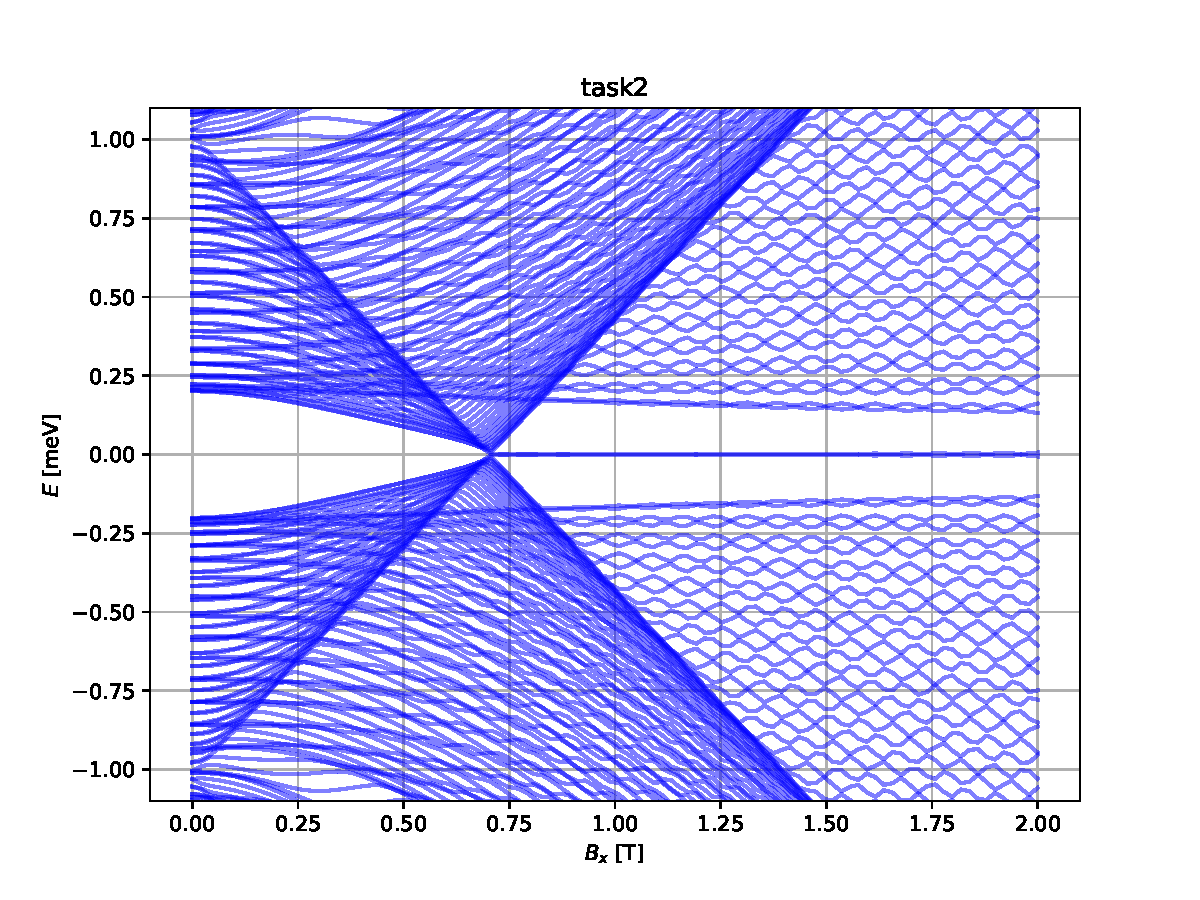
\includegraphics[width=0.65\linewidth]{task2_spectrum_vs_Bx.pdf}
    \caption{Spektrum energii w funkcji pola $B_x$. Wyniki dla realistycznego modelu nanodrutu z SOC}
    \label{fig:task2-spectra}
\end{figure}
%%%%%%%%%%%%%%%%%%%%%%%%%%%%%%%%%%%%%%%%%%%%%%%%%%%
Dla pola $B_x = 1$~T obserwujemy pojawienie się stanów o zerowej energii oraz lokalizację ich funkcji falowych na końcach nanodrutu, co świadczy o obecności stanów Majorany. \\
\\
W przypadku rotacji pola w płaszczyznach $xy$ i $xz$ spektrum wykazuje rozszczepienia zgodne z zachowaniem oczekiwanym w obecności silnego sprzężenia spin--orbita i nadprzewodnictwa (rys.~\ref{fig:energy-spectra-xy},~\ref{fig:denisty_xz}).
%%%%%%%%%%%%%%%%%%%%%%%%%%%%%%%%%%%%%%%%%%%%%%%%%%%
\begin{figure}[htp!]
    \centering
    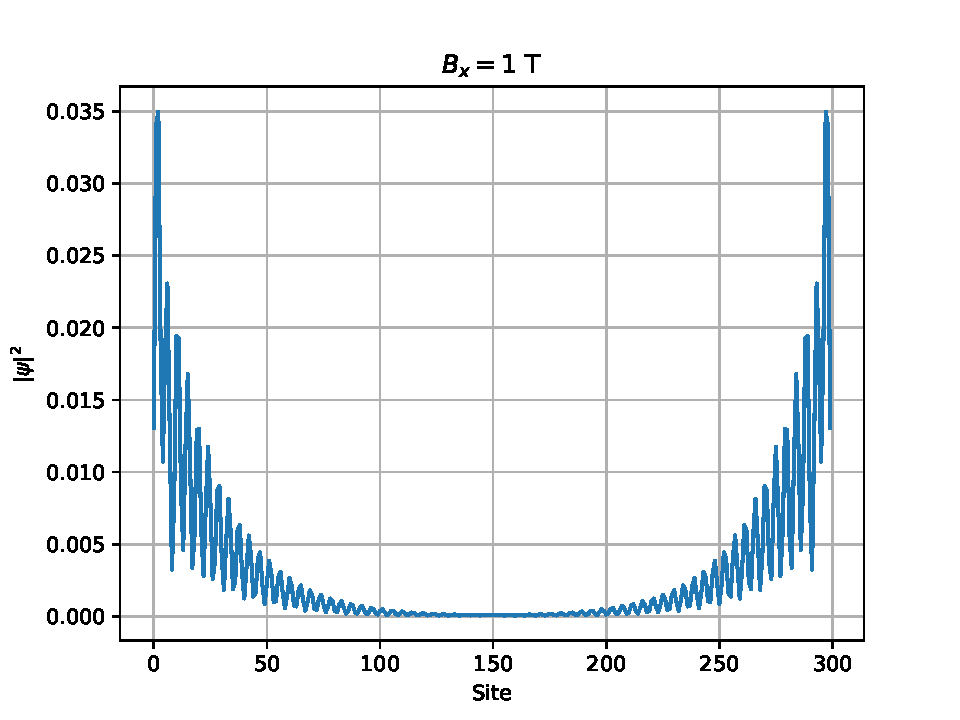
\includegraphics[width=0.65\linewidth]{task3_density_Bx1.pdf}
\caption{Moduł funkcji falowej w nanodrucie policzony dla realistycznego modeli nanodrutu z SOC. Wyniki dla $B_x = 1$~T dla stanu najbliższego energii $E = 0$}
    \label{fig:denisty-Bx}
\end{figure}
%%%%%%%%%%%%%%%%%%%%%%%%%%%%%%%%%%%%%%%%%%%%%%%%%%%
%%%%%%%%%%%%%%%%%%%%%%%%%%%%%%%%%%%%%%%%%%%%%%%%%%%
\begin{figure}[htp!]
    \centering
    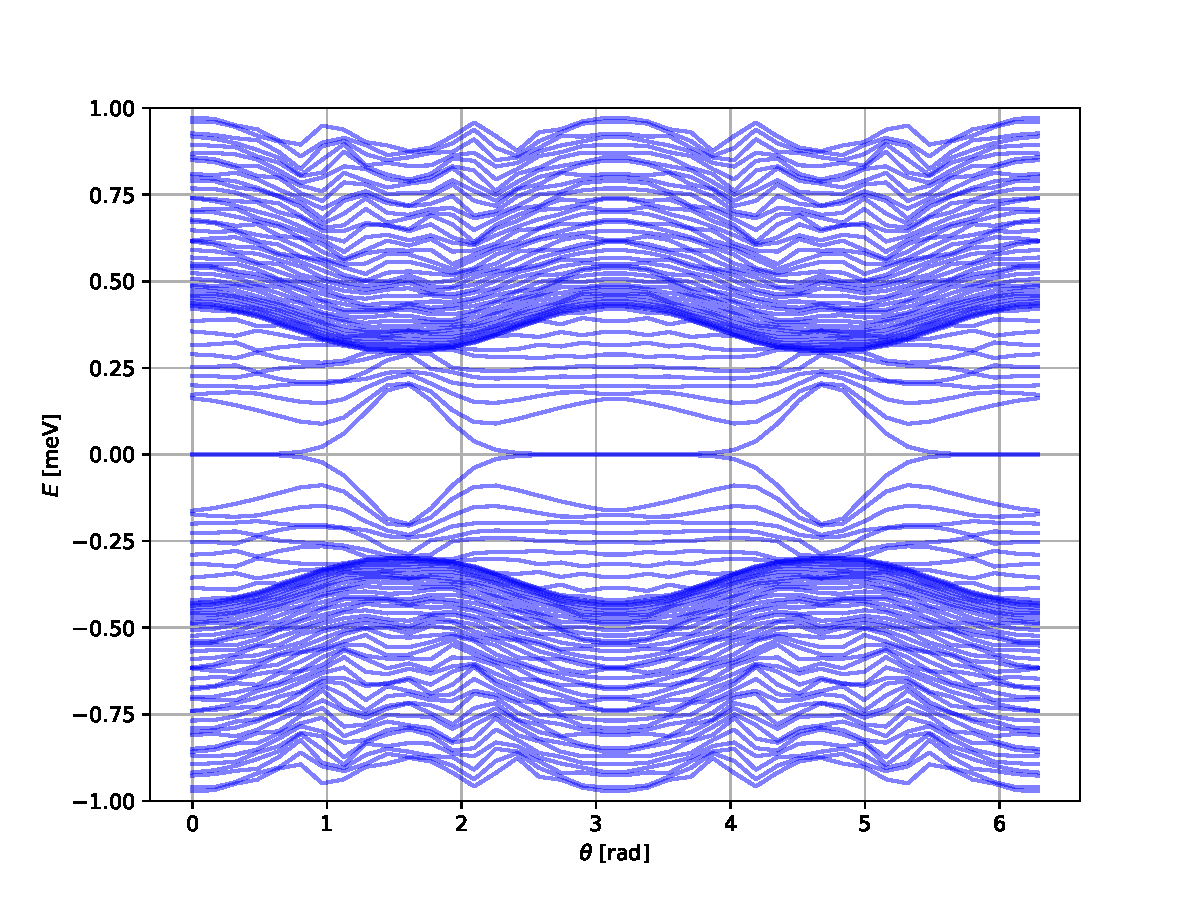
\includegraphics[width=0.65\linewidth]{task4_spectrum_vs_theta_xy.pdf}
\caption{Spektrum energii w funkcji pola rotującego w płaszczyźnie $xy$. Wyniki dla realistycznego modelu
nanodrutu z SOC, dla $|B| = 1$~T.}
    \label{fig:energy-spectra-xy}
\end{figure}
%%%%%%%%%%%%%%%%%%%%%%%%%%%%%%%%%%%%%%%%%%%%%%%%%%%
%%%%%%%%%%%%%%%%%%%%%%%%%%%%%%%%%%%%%%%%%%%%%%%%%%%
\begin{figure}[htp!]
    \centering
    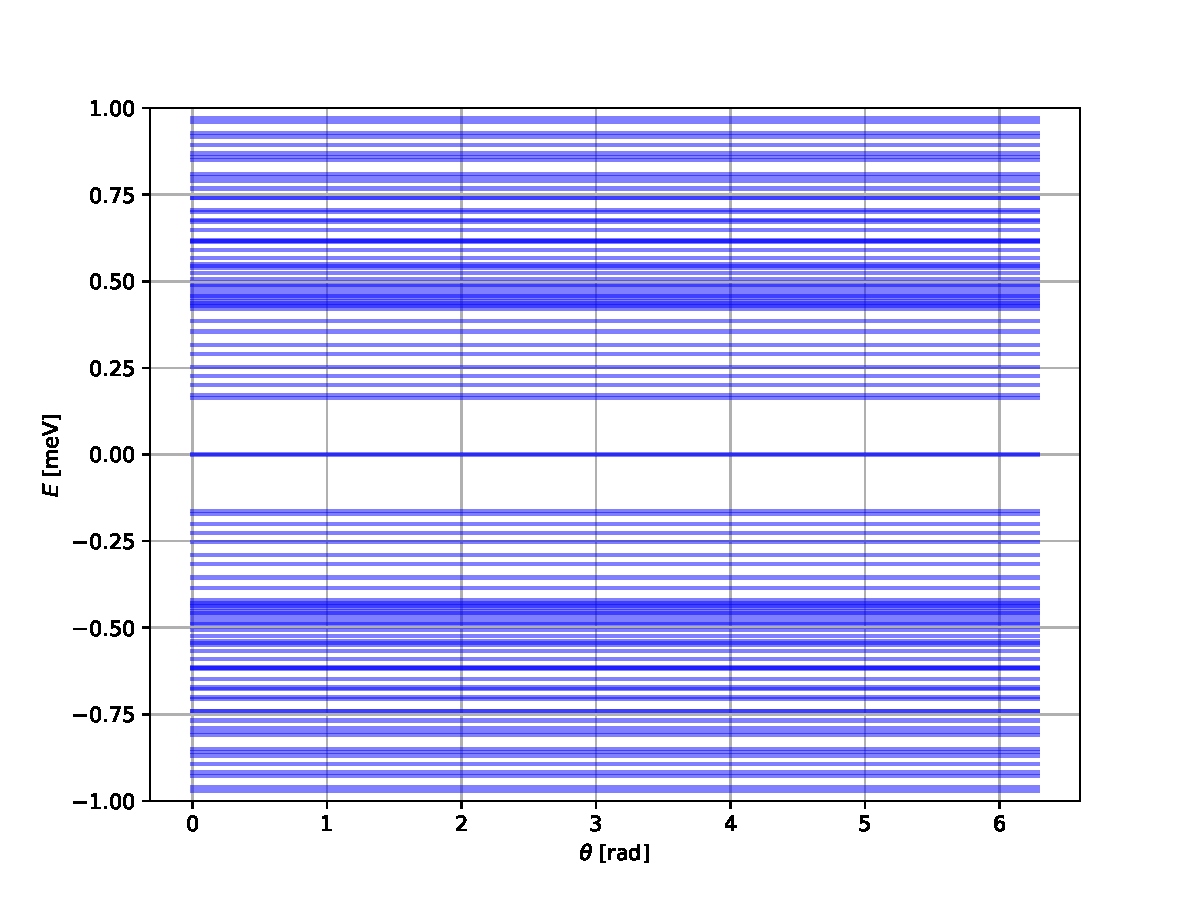
\includegraphics[width=0.65\linewidth]{task5_spectrum_vs_theta_xz.pdf}
\caption{: Spektrum energii w funkcji pola rotującego w płaszczyźnie $xz$. Wyniki dla realistycznego modelu
nanodrutu z SOC, dla $|B| = 1 $~T.}
    \label{fig:denisty_xz}
\end{figure}
%%%%%%%%%%%%%%%%%%%%%%%%%%%%%%%%%%%%%%%%%%%%%%%%%%%
\end{document}
